\questionheader{Question 5: Fixed versus Learnable Adjacency Matrices}

All three graphs use the same encoder, graph layer, head, splits, seed and training (Table 2).
\begin{itemize}
    \item \textbf{(a) Fixed:} The road graph is directed, so the symmetric normalisation would be wrong; each row is divided by its sum instead, so every sensor averages over the sensors it has edges to. The graph is a constant, not a trained weight, and is unchanged after training. Test MAE 60.92, RMSE 95.94, 382 s.
    \item \textbf{(b) Adaptive:} Each sensor gets two learned 10-number embeddings, initialised at random. Their pairwise similarity, with negative scores set to zero and a softmax over each row, gives a learned graph that is rebuilt in every forward pass and trained by backpropagation with the rest of the model. I keep the full graph (no top-$k$), which is cheap on the TPU. It is still concentrated: the 10 strongest links hold 70\% of each row on average. It has no road-like diagonal band (Figure 4). Test MAE improves by 12.2\% over the fixed graph, to 53.47.
    \item \textbf{(c) Hybrid:} A weighted mix of the fixed and learned graphs, both with rows summing to 1, where the mixing weight is learned (starting at 0.5). It settled at 0.026 on the road graph, so the model relies almost entirely on the learned graph. The hybrid is best on every metric (test MAE 51.09, 4.5\% below adaptive), though it also trained longer (100 vs 44 epochs).
\end{itemize}

\begin{center}
{\footnotesize\textbf{Figure 4: fixed row-normalised road graph (left) and learned adaptive graph (right); colours capped at the 99th percentile}}\\[2pt]
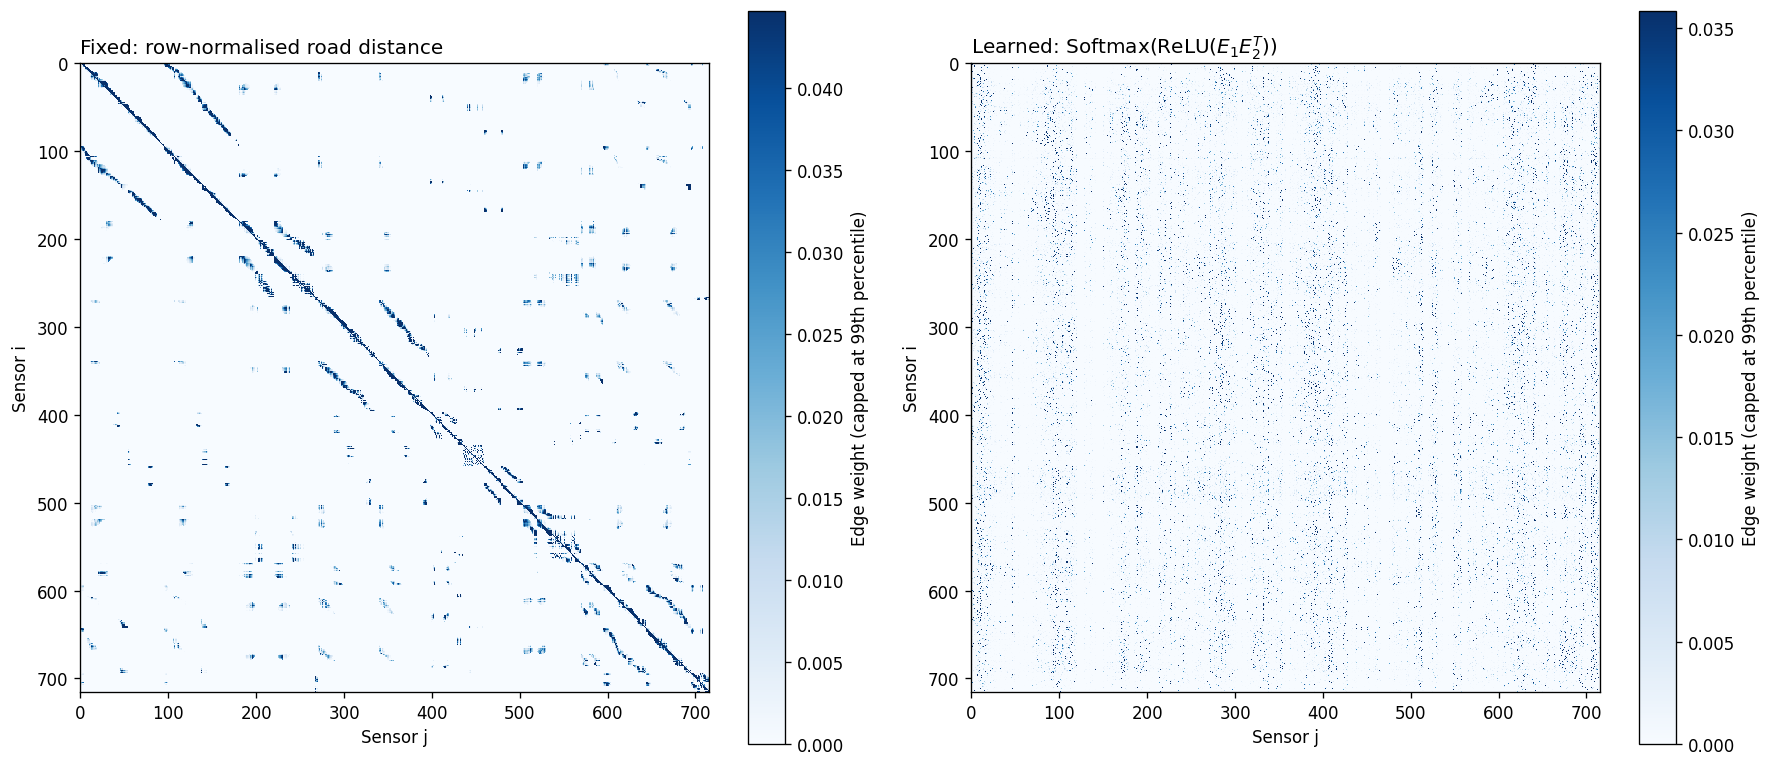
\includegraphics[width=0.86\textwidth]{figures/q5_adjacency.png}
\end{center}
